\subsection{High Level Parameterization}

The main program loop calculates the robot weight. This incorporates all calculations involving forces and component geometry, as both will vary with and influence the weight. The first components calculated are the Leg and Force object, which contain important properties such as the torque at joints and lengths of linkages. The springs are calculated before the shafts, as the shafts' lengths are dependent on the springs' length. The order of the remaining components has no impact on their calculations. The order was chosen based on which components are geometrically dependent and the order which enabled the most components to be fully defined at their initialization.

An initial weight prediction is given, and is either reduced or increased at each iteration as the estimate becomes more precise. Once the total weight of the robot varies by less than 1 kg, the program exits the main iteration cycle and prints the required properties to all text files. A high level flow chart for the parameterization of the O-Crab is shown in Figure \ref{fig:parametrization_flowchart}. For simplification, the exterior knee shaft is referred as knee shaft, the hip control shaft as hip shaft and knee control shaft as knee hip shaft.

\begin{figure}
    \centering
    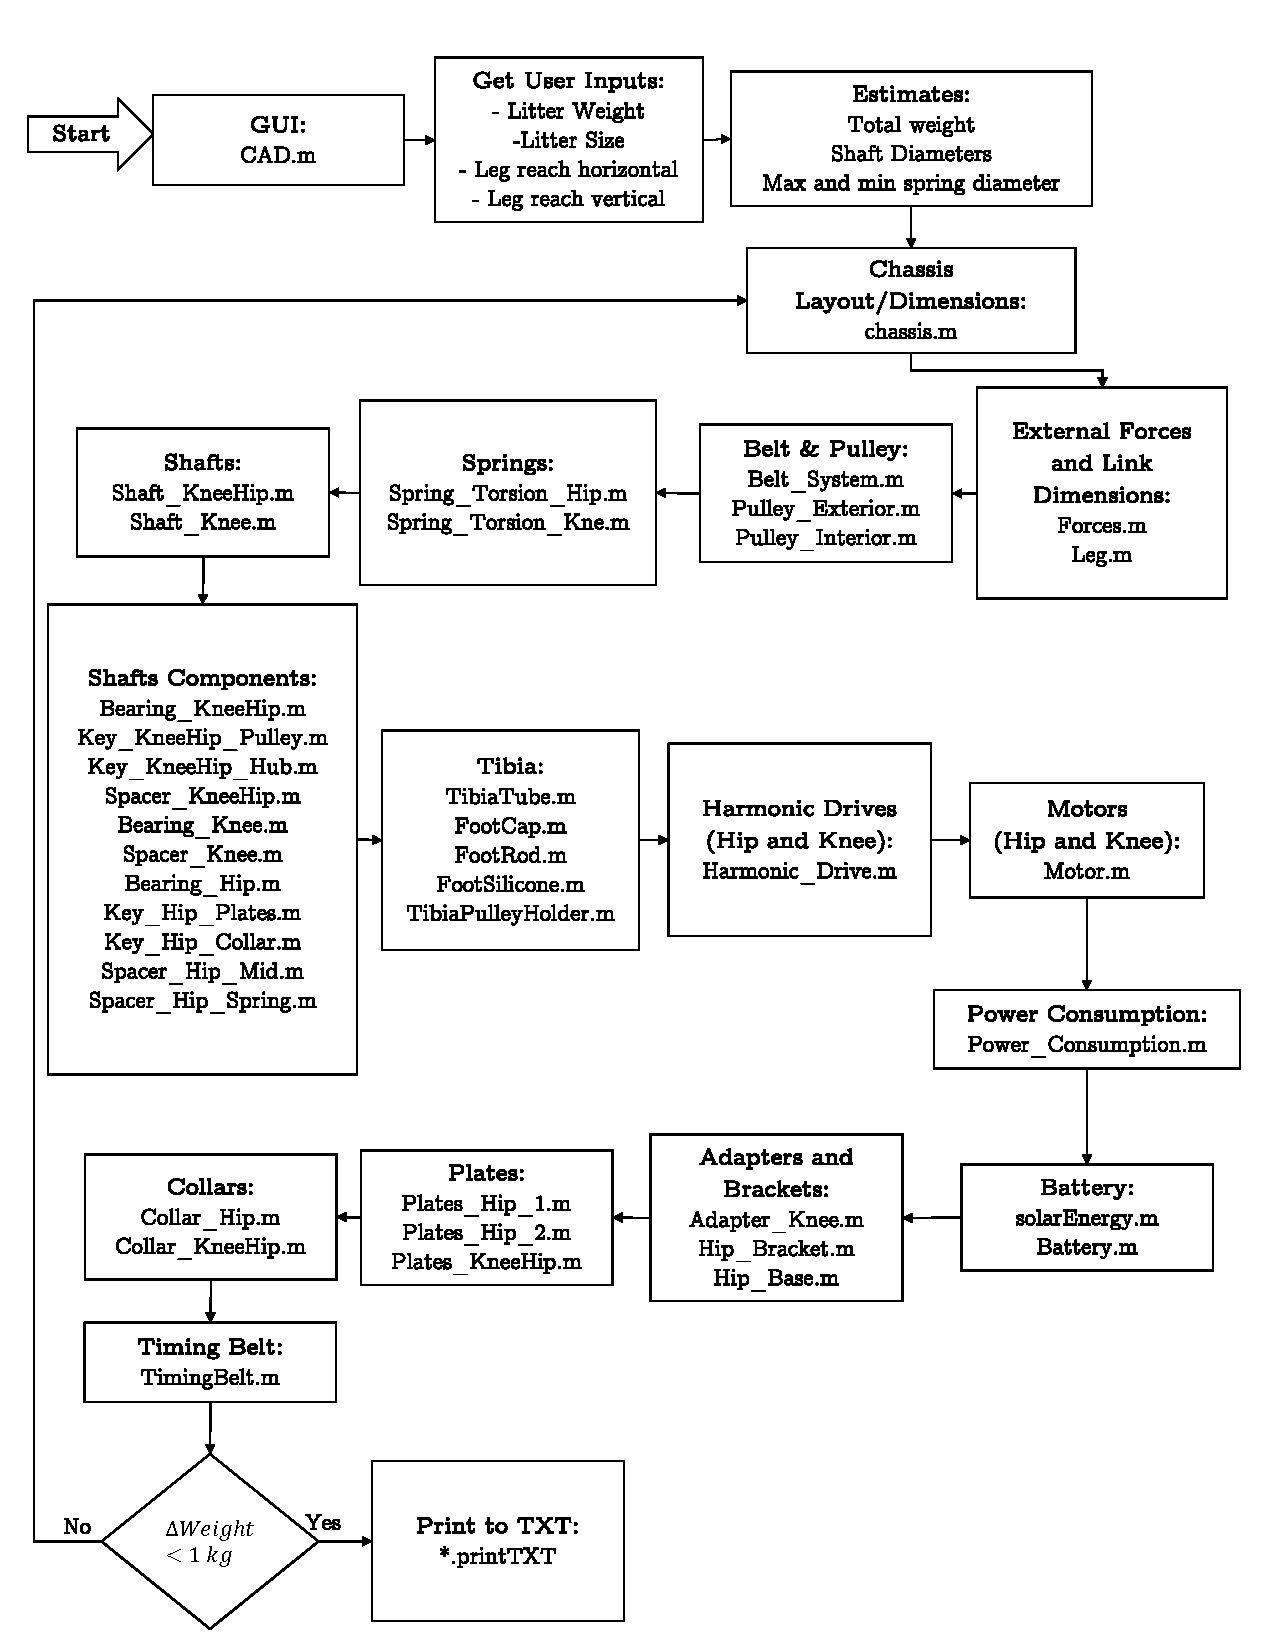
\includegraphics[width=\textwidth]{3_Parametrization/img/HighLevelFlowChart.pdf}
    \caption{Master parameterization flowchart}
    \label{fig:parametrization_flowchart}
\end{figure}{}